% =====================================================================
%  ME 697 -- Class Project extra credit: Reactive Burn, HVRB       v4
%  v4 (Oct 31, 2026, with Claude): citations completed -- DK's four
%  (Starkenberg IDS 2010; Stewart et al. IDS 2024; Ruggirello, Tuttle &
%  Kittell AIP CP 2023; Kittell et al. IDS 2018) plus Tuttle et al. (AIP
%  CP 2018, on the no-desensitization note) added and cited where
%  they support the sheet; bibitems in order of first citation; the red
%  'To place' line removed.  Cross-checks in README.md (ledger).  Also:
%  the red 'Confirm with the sweep' removed -- G2 (Oct 30) showed every
%  Material X cell burned to lambda = 1 behind the front at 1.00 and
%  1.25 km/s.  No other change from v3.  v3 notes follow.
%
%  Fall 2026, D. Kittell.  v3 drafted Oct 30, 2026 (with Claude) from v2,
%  after DK's two 2.00 km/s runs (fix-up off/on) and EOS checks A-C.
%  v1 (DK's notes) and v2 are kept unchanged.
%
%  STUB CONVENTION: \tbd{...} RED = still DK's decision or awaiting the
%  gold-standard sweep (GOLD_STANDARD_DATASET.md).  Black = verified.
%
%  WHAT v3 CHANGES (for DK to accept or reject)
%    [1] Layout for students: p1 what HVRB adds to a hydrocode (three
%        things) and the separable rate law; p2 the topology with a new
%        figure (hvrb_topology_v1.pdf); p3 the potential and the EOS pair;
%        p4 the closure and the algorithm; p5 parameters and checks;
%        p6 references.
%    [2] Temperature convention now matches DK's code (the reference
%        data): products energy zero at T = 0 K, e_gas = C_V T - Q, so
%        P_gas = (gamma-1) rho C_V T = (gamma-1) rho (e_gas + Q).  Closure:
%        C_V T = e - (1-lam)[e_S - C_V T_S] + lam Q.  With this convention
%        the scout code matches DK's arrival times to <= 4 ns at 100 zpm
%        (v2 convention, gas zero at T0: 5 ns; T-free closure: 9 ns).
%    [3] Parameters black, C_V = 1.16 J/(g K) = 1.35e11 erg/(g eV) (DK's
%        default; P is insensitive to C_V).  Verified in two codes.
%    [4] Algorithm box black: burn changes lambda at fixed rho and e, so
%        the energy update is the Hydrocode sheets' one; frozen-lambda
%        sound speed; reaction zone ~19 ns at CJ (exact ZND), about
%        0.14 mm of initial coordinate, ~5 cells at 35 zones/mm.
%    [5] Checks box: constant-volume burn to (gamma-1) rho0 Q = 12.50 GPa
%        (not a Sec. 7 answer); energy conserved while burning (the
%        lesson of DK's fix-up run); lambda rebuilt from a tracer's P
%        history; no detonation speed below D_CJ.
%    [6] Closure box: one line on why P can rise behind the shock (exact
%        ZND: P peaks near lambda = 0.5 at 36.8 GPa, above the 35.7 GPa
%        spike), and an optional T-free closure (red, DK's call).
%  STILL RED: lambda <-> Y_k line; project Sec. 4 "No temperature field";
%    whether to offer the T-free closure; the quench note and which
%    velocities detonate (await G2); missing citations.
%  NOT ON THE SHEET ON PURPOSE (project Sec. 7): D_CJ 7.500 km/s,
%    P_CJ 25.0 GPa, u_CJ 2.083 km/s, ZND spike 35.7 GPa.
% =====================================================================
\documentclass[11pt,addpoints]{exam}
\usepackage{amsfonts,amssymb,amsmath, amsthm}
\usepackage{graphicx}
\usepackage{enumitem}
\usepackage{systeme}
\usepackage{pgf,tikz,pgfplots}
\pgfplotsset{compat=1.15}
\usepgfplotslibrary{fillbetween}
\usepackage{mathrsfs}
\usepackage{multicol}
\usepackage{booktabs}
\usepackage[many]{tcolorbox}
\usepackage{bm}
\usepackage{cancel}
\allowdisplaybreaks

% Good Volume Symbol
\newcommand{\volume}{{\ooalign{$V$\cr\hfil\raisebox{0.35em}{\rule{2.1mm}{0.1ex}}\hfil\cr}}}

%%% Strike-out font
\usepackage{ulem}
\normalem
\pagestyle{headandfoot}

% ---- Warm theme to match the figures (U5 onward) ----
\definecolor{slate}{HTML}{2C3E50}
\definecolor{oiblue}{HTML}{0072B2}
\tcbset{colback=oiblue!4!white, colframe=slate, boxrule=0.5pt, arc=1.5mm}

% ---- Stub marker: red = placeholder (delete when the sheet is final) ----
\newcommand{\tbd}[1]{\textcolor{red}{#1}}

\firstpageheader{ME 697 Equations}{Class Project: Reactive Burn, HVRB}{Fall 2026 -- D. Kittell}
\runningheader{ME 697 Equations}{Class Project: Reactive Burn, HVRB}{Fall 2026 -- D. Kittell}
\runningheadrule
\firstpagefooter{}{}{}
\runningfooter{}{}{}

\makeatletter
\renewcommand*\env@matrix[1][*\c@MaxMatrixCols c]{%
  \hskip -\arraycolsep
  \let\@ifnextchar\new@ifnextchar
  \array{#1}}
\makeatother



\begin{document}

\noindent
\bf{Instructor's Note:}\normalfont\\

\noindent
\it{Extra credit for the class project (Sec.~9, +10 points). The History Variable Reactive Burn (HVRB) model of G.~I.~Kerley is pressure-based, simple and robust, and in widespread use; it adds one progress variable and one closure rule to the hydrocode you already have. Nothing on this sheet is required, and skipping it costs you nothing.}\normalfont\vspace{1.5em}

\textbf{These equations build upon U3. Continuum Mechanics {\&} Balance Laws and the Class Project: Hydrocode sheets (Method AV and Method RS)}\vspace{1em}


\begin{tcolorbox}[breakable]
\textbf{What HVRB Adds to Your Hydrocode:}\vspace{.5em}
\begin{itemize}
\item A progress variable, \hspace{3mm} \bm{$\lambda$}, \hspace{2mm} in every Material X cell: \hspace{2mm} \bm{$\lambda=0$} unreacted, \bm{$\lambda=1$} fully reacted \hspace{3mm} (carried with the cell; a Lagrangian mesh needs no advection)\vspace{.5em}
\item A rate law, \hspace{3mm} pressure history \bm{$\rightarrow$} \bm{$\lambda$} \hspace{7mm} pages 1--3\vspace{.5em}
\item A closure, \hspace{3mm} \bm{$\left(\rho,\;e,\;\lambda\right)\rightarrow P$} \hspace{7mm} page 4\vspace{.5em}
\item Notation, \hspace{3mm} history variable \bm{$\phi$}, \hspace{2mm} reaction potential \bm{$\Phi$}, \hspace{2mm} topology function \bm{$g\left(\lambda\right)$}; \hspace{2mm} phases \bm{$\left(\;\;\right)_{\text{solid}}$} and \bm{$\left(\;\;\right)_{\text{gas}}$}; \hspace{2mm} time level \bm{$n$}\vspace{.5em}
\item This \bm{$\lambda$} is not the U7 wave speed \bm{$\lambda_i$}, nor the U4 Lam\'e constant (it is the mass fraction of reaction product/gas, more closely related to U3's \bm{$Y_k$}, \bm{${\dot\Omega}_k$}, and \bm{$Q_k$})
% \hspace{3mm} \tbd{relation to U3: \bm{$\lambda$} in terms of \bm{$Y_k$}, \bm{${\dot\Omega}_k$}, \bm{$Q_k$}, one line}\vspace{.5em}
\item \textbf{\emph{Everything else in your cycle is unchanged}}
\end{itemize}
\end{tcolorbox}


\begin{tcolorbox}[breakable]
\textbf{Rate Law --- Separable, History-Variable Form:}\vspace{.5em}
\begin{itemize}
\item Separable assumption, \hspace{3mm} \bm{$\displaystyle \frac{D\lambda}{Dt}\;=\;g\left(\lambda\right)\,\Phi\left(P\right)$} \hspace{5mm} \bm{$g$} depends on \bm{$\lambda$} alone, \bm{$\Phi$} not on \bm{$\lambda$}\vspace{1.0em}
\item History variable, \hspace{3mm} \bm{$\displaystyle \phi\left(t\right)\;=\;\int_{0}^{t}\Phi\,d\hat{t}$} \hspace{5mm} so that \hspace{3mm} \bm{$\displaystyle g\left(\lambda\right)\;=\;\frac{d\lambda}{d\phi}$}\vspace{1.0em}
\item Inversion, \hspace{3mm} \bm{$\displaystyle \phi\;=\;F\left(\lambda\right)\;=\;\int_{0}^{\lambda}\frac{d\hat{\lambda}}{g\left(\hat{\lambda}\right)}$} \hspace{5mm} and \hspace{3mm} \bm{$\displaystyle \lambda\;=\;F^{-1}\left(\phi\right)$}\vspace{.5em}
\item \textbf{\emph{The extent of reaction depends only on the accumulated pressure history, \bm{$\phi$}, not on how the pressure was delivered}}
\end{itemize}
\end{tcolorbox}




\clearpage

\begin{tcolorbox}[breakable]
\textbf{HVRB Topology (\bm{$M_R$}, \bm{$X_R$}) \cite{starkenberg2002,starkenberg2010,stewart2024,kittell2025sand}, Fig.~\ref{fig:hvrb-topology}:}\vspace{.5em}
\begin{itemize}
\item Extent of reaction, \hspace{3mm} \bm{$\displaystyle \lambda\;=\;1\;-\;\left(1\;-\;\frac{\phi^{M_R}}{X_R}\right)^{X_R}$} \hspace{5mm} for \bm{$\displaystyle 0\le\phi\le\phi_{end}\;=\;X_R^{1/M_R}$}, \hspace{2mm} then \bm{$\lambda=1$}\vspace{1.0em}
\item History variable, \hspace{3mm} \bm{$\displaystyle \phi\;=\;\left[X_R\left(1\;-\;\left(1-\lambda\right)^{1/X_R}\right)\right]^{1/M_R}$}\vspace{1.0em}
\item Topology function, \hspace{3mm} \bm{$\displaystyle g\left(\lambda\right)\;=\;\frac{d\lambda}{d\phi}$}\vspace{.5em} \\
.~~~~~~~~~~\bm{$\displaystyle =\;M_R\,X_R^{\,1-1/M_R}\left(1-\lambda\right)^{1-1/X_R}\left[1-\left(1-\lambda\right)^{1/X_R}\right]^{1-1/M_R}$}\vspace{1.0em}
\item Shape, \hspace{3mm} \bm{$g\left(0\right)=0$} needs \bm{$M_R>1$} (a delay behind the shock); \hspace{2mm} \bm{$g\left(1\right)=0$} needs \bm{$X_R>1$} (a gradual finish)
\end{itemize}
\end{tcolorbox}

\begin{figure}[h!]
  \centering
  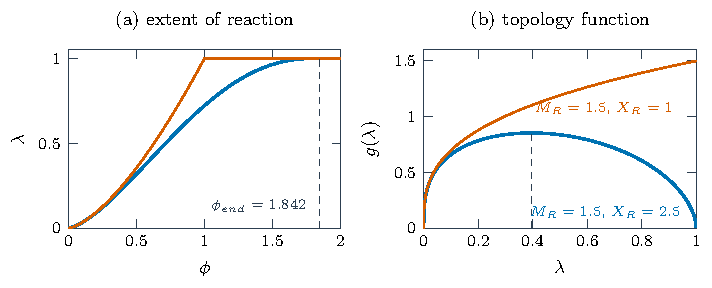
\includegraphics[width=0.80\textwidth]{hvrb_topology_v1.pdf}
  \caption{HVRB topology, exact curves. (a) \bm{$\lambda\left(\phi\right)$}; (b) \bm{$g\left(\lambda\right)=d\lambda/d\phi$}. Blue: the Material X set, \bm{$M_R=1.5$}, \bm{$X_R=2.5$}, with \bm{$g$} peaking at \bm{$\lambda=0.394$} (\bm{$g_{max}=0.854$}) and the burn complete at \bm{$\phi_{end}=1.842$}. Orange: \bm{$M_R=1.5$}, \bm{$X_R=1$}, common input defaults; \bm{$g$} never returns to zero and the burn stops abruptly at \bm{$\phi=1$}.}
  \label{fig:hvrb-topology}
\end{figure}


\clearpage

\begin{tcolorbox}[breakable]
\textbf{HVRB Reaction Potential (\bm{$P_R$}, \bm{$Z_R$}, \bm{$P_I$}, \bm{$\tau_0$}) \cite{starkenberg2010,stewart2024}:}\vspace{.5em}
\begin{itemize}
\item Potential, \hspace{3mm} \bm{$\displaystyle \Phi\;=\;\frac{1}{\tau_0}\left[\frac{{\max}\left(P-P_I,\;0\right)}{P_R}\right]^{Z_R}$} \hspace{5mm} \bm{$P$} is the cell's mixture pressure, \bm{$P^n$}\vspace{1.0em}
\item \bm{$\phi$} grows only while \bm{$P>P_I$} and never decreases; \hspace{2mm} \bm{$\tau_0=1$} \bm{$\mu$}s by convention (not \bm{$10^{-6}$} in \bm{$\mu$}s units)\vspace{.5em}
\item Only the product \bm{$\tau_0P_R^{\,Z_R}$} enters: \hspace{2mm} changing \bm{$\tau_0$} is the same as rescaling \bm{$P_R$} by \bm{$\tau_0^{\,1/Z_R}$} \hspace{3mm} \cite{starkenberg2014}\vspace{.5em}
\item \textbf{\emph{HVRB cannot quench and cannot desensitize: any cell held above \bm{$P_I$} eventually burns}} \cite{tuttle2018}\textbf{\emph{.}}
\end{itemize}
\end{tcolorbox}




\begin{tcolorbox}[breakable]
\textbf{Unreacted Material X (Mie--Gr\"uneisen, from the project):}\vspace{.5em}
\begin{itemize}
\item Pressure, \hspace{3mm} \bm{$\displaystyle P_{\text{solid}}\left(\text{V},e\right)\;=\;\rho_0\Gamma_0\,e\;+\;\left[\frac{1}{\text{V}_0-\text{V}}\;-\;\frac{1}{2}\rho_0\Gamma_0\right]u_p^2$} \hspace{5mm} project Eq.~(4), \bm{$\Gamma\rho=\Gamma_0\rho_0$}\vspace{1.0em}
\item Principal isentrope, \hspace{3mm} \bm{$\displaystyle \frac{de_S}{d\text{V}}\;=\;-P_{\text{solid}}\left(\text{V},e_S\right)$}, \hspace{2mm} \bm{$e_S\left(\text{V}_0\right)=0$}; \hspace{5mm} \bm{$\displaystyle T_S\;=\;T_0\,{\exp}\left(\Gamma_0\eta\right)$}\vspace{1.0em}
\item Temperature, \hspace{3mm} \bm{$\displaystyle e_{\text{solid}}\;=\;e_S\left(\text{V}\right)\;+\;C_\text{V}\left[T-T_S\left(\text{V}\right)\right]$} \hspace{5mm} \bm{$e=0$}, \bm{$T=T_0$} at rest\vspace{.5em}
\item Here \bm{$T$} is only an intermediate result that is needed by the closure rule
\end{itemize}
\end{tcolorbox}


\begin{tcolorbox}[breakable]
\textbf{Detonation Products (constant \bm{$\gamma$}, from the project):}\vspace{.5em}
\begin{itemize}
\item Pressure, \hspace{3mm} \bm{$\displaystyle P_{\text{gas}}\;=\;\left(\gamma-1\right)\rho\left(e_{\text{gas}}+Q\right)$} \hspace{5mm} \bm{$\gamma=2s_1-1=2.60$}, \hspace{2mm} \bm{$Q=4.8828$} MJ/kg, \hspace{2mm} project Eq.~(8)\vspace{1.0em}
\item Temperature, \hspace{3mm} \bm{$\displaystyle e_{\text{gas}}\;=\;C_\text{V}T\;-\;Q$} \hspace{5mm} so \hspace{3mm} \bm{$\displaystyle P_{\text{gas}}\;=\;\left(\gamma-1\right)\rho\,C_\text{V}T$}\vspace{1.0em} 
\item Same \bm{$C_\text{V}$} as the solid, for simplicity's sake in your hydrocode
\end{itemize}
\end{tcolorbox}


\clearpage

\begin{tcolorbox}[breakable]
\textbf{Mixture Closure (density--temperature equilibrium) \cite{ruggirello2023,kittell2018}:}\vspace{.5em}
\begin{itemize}
\item Both phases at the same cell density \bm{$\rho$} and temperature \bm{$T$}; \hspace{2mm} the solid and gas phase pressures differ \hspace{3mm} (pressure--temperature equilibrium is the common alternative \cite{ruggirello2023})\vspace{.5em}
\item Pressure, \hspace{3mm} \bm{$\displaystyle P\;=\;\left(1-\lambda\right)P_{\text{solid}}\left(\rho,T\right)\;+\;\lambda\,P_{\text{gas}}\left(\rho,T\right)$}\vspace{.5em}
\item Energy, \hspace{3mm} \bm{$\displaystyle e\;=\;\left(1-\lambda\right)e_{\text{solid}}\left(\rho,T\right)\;+\;\lambda\,e_{\text{gas}}\left(\rho,T\right)$}\vspace{.5em}
\item One \bm{$C_\text{V}$}: the energy line is linear in \bm{$T$}, so given \bm{$\left(\rho,\;e,\;\lambda\right)$} there is no iteration:\vspace{.5em} \\
.~~~~~~~~~~\bm{$\displaystyle C_\text{V}T\;=\;e\;-\;\left(1-\lambda\right)\left[e_S\left(\text{V}\right)-C_\text{V}T_S\left(\text{V}\right)\right]\;+\;\lambda\,Q$}\vspace{.5em}
\item Limits, \hspace{3mm} \bm{$\lambda=0$} returns \bm{$P_{\text{solid}}\left(\text{V},e\right)$}; \hspace{2mm} \bm{$\lambda=1$} returns \bm{$\left(\gamma-1\right)\rho\left(e+Q\right)$}\vspace{.5em}
\item Compressed solid is stiffer than gas at equal \bm{$\rho$} and \bm{$T$}, so early burning can \emph{raise} the pressure behind the shock\vspace{.5em}
\item Same closure algorithm without using \bm{$T$} (exact, since both phases share one \bm{$C_\text{V}$}): \hspace{2mm} let \bm{$\vartheta\equiv C_\text{V}T$} and the solid's \bm{$T=0$} `cold' curve,\vspace{.5em} \\
.~~~~~~~~~~\bm{$\displaystyle e_c\left(\text{V}\right)\;=\;e_S\left(\text{V}\right)-C_\text{V}T_S\left(\text{V}\right)$}, \hspace{5mm} \bm{$\displaystyle P_c\left(\text{V}\right)\;=\;P_{\text{solid}}\left(\text{V},e_S\right)-\rho_0\Gamma_0C_\text{V}T_S\left(\text{V}\right)$}\vspace{.5em} \\
.~~~~~~~~~~\bm{$\displaystyle \vartheta\;=\;e\;-\;\left(1-\lambda\right)e_c\left(\text{V}\right)\;+\;\lambda\,Q$}\vspace{.5em} \\
.~~~~~~~~~~\bm{$\displaystyle P\;=\;\left(1-\lambda\right)\left[P_c\left(\text{V}\right)+\rho_0\Gamma_0\vartheta\right]\;+\;\lambda\left(\gamma-1\right)\rho\,\vartheta$}
\end{itemize}
\end{tcolorbox}




\begin{tcolorbox}[breakable]
\textbf{Adding Burn to One Cycle (Lagrangian, Method AV or RS):}\vspace{.5em}
\begin{itemize}
\item After momentum, position, volume and energy, for each Material X cell:\vspace{.5em}
\item Potential, \hspace{3mm} \bm{$\Phi^n$} from \bm{$P^n$}; \hspace{5mm} history, \hspace{3mm} \bm{$\displaystyle \phi^{n+1}\;=\;{\min}\left(\phi^n\;+\;\Phi^n\,\Delta t^n,\;\;\phi_{end}\right)$}\vspace{.5em}
\item Progress, \hspace{3mm} \bm{$\displaystyle \lambda^{n+1}\;=\;F^{-1}\left(\phi^{n+1}\right)$} \hspace{5mm} exact; \bm{$0\le\lambda\le 1$} automatically\vspace{.5em}
\item Pressure, \hspace{3mm} closure with \bm{$\left(\rho^{n+1},\;e^{n+1},\;\lambda^{n+1}\right)$}; \hspace{2mm} then \bm{$q$} and \bm{$\Delta t$} as usual\vspace{.5em}
\item Burning changes \bm{$\lambda$} at fixed \bm{$\rho$} and \bm{$e$}: \hspace{2mm} the energy update is the one on the Hydrocode sheets, and total energy must stay conserved\vspace{.5em}
\item Time step, \hspace{3mm} the mixture sound speed at fixed \bm{$\lambda$} in the CFL condition\vspace{.5em}
\item Zoning, \hspace{3mm} the steady reaction zone lasts \bm{$\approx 19$} ns, \bm{$\approx 0.14$} mm of initial coordinate: \hspace{2mm} \bm{$\approx 5$} cells at 35 zones/mm\vspace{.5em}
\item \textbf{\emph{The stiff part, \bm{$g\left(\lambda\right)$}, is integrated exactly; the only error is the first-order quadrature of \bm{$\Phi$}}}
\end{itemize}
\end{tcolorbox}


\clearpage

\begin{tcolorbox}[breakable]
\textbf{Mixture Sound Speed (fixed \bm{$\lambda$}):}\vspace{.5em}
\begin{itemize}
\item Phases, \hspace{3mm} \bm{$c_{\text{solid}}$}: inert Mie--Gr\"uneisen at \bm{$\left(\text{V},\,e_c+\vartheta\right)$}; \hspace{3mm} \bm{$c_{\text{gas}}^2=\gamma\left(\gamma-1\right)\vartheta$}\vspace{.5em}
\item Mass-weighted, \hspace{3mm} \bm{$\displaystyle c^2\;\approx\;\left(1-\lambda\right)c_{\text{solid}}^2\;+\;\lambda\,c_{\text{gas}}^2$} \hspace{5mm} recommended, \bm{$\approx 1\%$} high\vspace{.5em}
\item Exact, \hspace{3mm} subtract \bm{$\displaystyle \lambda\left(1-\lambda\right)\left(\rho_0\Gamma_0/\rho-\gamma+1\right)^2\vartheta$} \hspace{5mm} (the spread of the two \bm{$\Gamma$}'s)\vspace{.5em}
\item Schmidt, \hspace{3mm} \bm{$Z^{-2}=\left(1-\lambda\right)Z_{\text{solid}}^{-2}+\lambda Z_{\text{gas}}^{-2}$}, \bm{$Z=\rho c$}; \hspace{2mm} equal-\emph{pressure} rule, \bm{$\approx 15\%$} low\vspace{.5em}
\item \textbf{\emph{The sound speed sets only \bm{$\Delta t$} and \bm{$q$}, not the converged solution}}
\end{itemize}
\end{tcolorbox}


\begin{tcolorbox}[breakable]
\textbf{HVRB Parameters for Material X (notional):}\vspace{.5em}

\begin{center}
\begin{tabular}{lcc}
\toprule
\textbf{Parameter} & \textbf{Value} & \textbf{Units} \\
\midrule
\bm{$P_R$}, reference pressure      & 7.0  & GPa \\
\bm{$Z_R$}, pressure exponent        & 3.0  & -- \\
\bm{$M_R$}, delay exponent           & 1.5  & -- \\
\bm{$X_R$}, completion exponent      & 2.5  & -- \\
\bm{$P_I$}, threshold pressure       & 1.0  & GPa \\
\bm{$\tau_0$}, time constant         & 1.0  & \bm{$\mu$}s \\
\bm{$C_\text{V}$}, both phases       & 1.16 & J/(g\,K) \\
\bm{$T_0$}, initial temperature      & 298  & K \\
\bottomrule
\end{tabular}
\end{center}
\end{tcolorbox}


\begin{tcolorbox}[breakable]
\textbf{Checks Before the Velocity Sweep:}\vspace{.5em}
\begin{itemize}
\item Inert limit, \hspace{3mm} \bm{$\Phi\equiv 0$} reproduces your inert PDV trace exactly\vspace{.25em}
\item Constant-volume burn, \hspace{3mm} one cell at rest, \bm{$\lambda$}: \bm{$0\rightarrow 1$} at fixed \bm{$e$}, \hspace{2mm} ends at \bm{$P=\left(\gamma-1\right)\rho_0Q=12.50$} GPa\vspace{.25em}
\item Energy, \hspace{3mm} total energy conserved to \bm{$\lesssim 0.01\%$} while Material X burns\vspace{.25em}
\item HVRB, \hspace{3mm} \bm{$\lambda$} rebuilt from one tracer's \bm{$P\left(t\right)$} history with the two HVRB boxes matches your \bm{$\lambda\left(t\right)$}\vspace{.25em}
\item Detonation, \hspace{3mm} the shock speed never settles below your \bm{$D_{CJ}$} from project Sec.~7\vspace{.25em}
\item Pop plot, \hspace{3mm} run distance versus input pressure is a straight line on log--log axes \cite{ramsay1965}\vspace{.25em}
\item Sweep, \hspace{3mm} 2.00, 1.75, 1.50 km/s detonate (run \bm{$\approx$} 3.5, 5.5, 7.5 mm); \hspace{2mm} 1.25, 1.00 km/s do not within 10 mm (late PDV wave only)
\end{itemize}
\end{tcolorbox}


\clearpage

\begin{tcolorbox}[breakable]
\textbf{References:}\vspace{.5em}

% Ledger: README.md in this folder.  One \bibitem per ledger row, same key.
\begingroup
\renewcommand{\section}[2]{}% suppress the "References" heading inside the box
\begin{thebibliography}{9}
\setlength{\itemsep}{0.25em}
\bibitem{starkenberg2002}
J.~Starkenberg, ``Modeling detonation propagation and failure using explosive initiation models in a conventional hydrocode,'' in \emph{Proceedings of the 12th International Detonation Symposium}, San Diego, CA (2002), pp.~1001--1007.
\bibitem{starkenberg2010}
J.~Starkenberg, ``Adaptation of an explosive initiation model for treatment of short-pulse and multiple shock wave loading,'' in \emph{Proceedings of the Fourteenth International Detonation Symposium}, Office of Naval Research, ONR 351-10-185 (2010), pp.~1497--1503.
\bibitem{stewart2024}
J.~A. Stewart, D.~E. Kittell, A.~S. Tappan, R.~A. Knepper, D.~L. Damm, W.~P. Bassett, and L.~W. Tuttle, ``Reactive burn model calibration for vapor deposited hexanitrostilbene and pentaerythritol tetranitrate films using XHVRB,'' in \emph{Proceedings of the 17th International Detonation Symposium}, edited by W.~A. Bagley III (Energetics Research Group, Johns Hopkins University, Kansas City, MO, 2024), pp.~998--1003.
\bibitem{kittell2025sand}
D.~E. Kittell \emph{et al.}, ``A Short Survey of Current Reactive Burn Model Capabilities as of Mid-Year 2025,'' Sandia National Laboratories, SAND2025-09228 (July 2025).
\bibitem{starkenberg2014}
J.~Starkenberg, ``Shock-pressure and pseudo-entropic approaches to explosive initiation modeling,'' in \emph{Proceedings of the Fifteenth International Detonation Symposium}, Office of Naval Research, ONR 43-280-15 (2014), pp.~908--916.
\bibitem{tuttle2018}
L.~W. Tuttle, R.~G. Schmitt, D.~E. Kittell, and E.~N. Harstad, ``Evaluation of XHVRB for capturing shock desensitization,'' \emph{AIP Conf.\ Proc.} \textbf{1979} (2018), doi:10.1063/1.5044916.
\bibitem{ruggirello2023}
K.~P. Ruggirello, L.~W. Tuttle, and D.~E. Kittell, ``Comparison of reactive burn equilibrium closure assumptions in CTH,'' \emph{AIP Conf.\ Proc.} \textbf{2844}, 300016 (2023), doi:10.1063/12.0020384.
\bibitem{kittell2018}
D.~E. Kittell, R.~G. Schmitt, L.~W. Tuttle, and E.~N. Harstad, ``Implementation of a CREST multistate reactive burn model in CTH for two solid high explosives,'' in \emph{Proceedings of the Sixteenth International Detonation Symposium}, ONR-43-5762-19 (2018), pp.~1021--1031.
\bibitem{ramsay1965}
J.~B. Ramsay and A.~Popolato, ``Analysis of shock wave and initiation data for solid explosives,'' in \emph{Fourth Symposium (International) on Detonation}, Office of Naval Research, ACR-126 (1965), pp.~233--238.
\end{thebibliography}
\endgroup
\end{tcolorbox}

\end{document}
